\documentclass[a4paper,10pt]{article}
\usepackage{jheppub} % for details on the use of the package, please see the JINST-author-manual
\usepackage{lineno}
\usepackage{amsmath,amsthm,amsfonts,amssymb,amscd,physics,cancel,mathtools}
\usepackage{tcolorbox}
\usepackage{marginnote,tensor}
%~~~~~~~~~ Document setup
% \usepackage[spanish]{babel} % English formatting
\usepackage[utf8]{inputenc} % Standard encoding
% \usepackage[a4paper,left=3cm,bottom=3cm]{geometry} % Page formatting
\usepackage{indentfirst} % Indents the first paragraph
\usepackage{amsmath} % Maths type package
\usepackage{bm} % Bold font maths
\usepackage{graphicx} % Advanced graphics package
\usepackage[export]{adjustbox} 
\usepackage{pdflscape} % Make pages landscape
\usepackage{fancyhdr} % Fancy headers
% \usepackage[colorlinks=true,citecolor=blue,urlcolor=blue,linkcolor=black]{hyperref} % Link colours
%\usepackage{natbib} % Bibliography
% \usepackage{flafter} % Reference any 'float'
% \usepackage[framemethod=tikz]{mdframed} % Box off stuff
\usepackage{color} % Colour support
\usepackage{wrapfig} % Text flowing around figures
\usepackage{lipsum} % Generates meaningless text
\usepackage{xcolor}
%\usepackage{biblatex}
%\usepackage[backend=bibtex]{biblatex}
%\addbibresource{bibliography.bib}
%\hypersetup{colorlinks=true, linkcolor=blue}

\theoremstyle{definition}
\newtheorem{ej}{Ejemplo}[section]
\newtheorem{sol}{Solución}[section]
\newtheorem{dem}{Demostración}[section]
\newtheorem{cor}{Corolario}[section]
\newtheorem{post}{Postulado}

\def\a{\alpha}
\def\b{\beta}
\def\g{\gamma}
\def\G{\Gamma}
\def\d{\delta}
%\def\D{\Delta}
%\def\e{\eta}
\def\la{\lambda}
\def\La{\Lambda}
\def\k{\kappa}
\def\m{\mu}
\def\n{\nu}
\def\r{\rho}
\def\p{\rho}
\def\o{\omega}
\def\s{\sigma}
\def\S{\Sigma}
\def\t{\tau}
\def\p{\pi}
\def\f{\phi}
\def\vf{\varphi}
\def\ep{\epsilon}
\def\th{\theta}
\def\Th{\Theta}
\def\z{\zeta}
\def\zc{z_{\rm C}}
\def\zgc{z_{\rm GC}}
\def\ogc{\omega_{\rm GC}}
\def\Ogc{\Omega_{\rm GC}}

\newcommand{\summ}{\sum_{i=1}^m}


%-----COLORS LIST ------
\definecolor{azure(colorwheel)}{rgb}{0.0, 0.5, 1.0}
\definecolor{DarkViolet}{RGB}{148,0,211}
\definecolor{myDarkBlue}{rgb}{0,0.1,0.7}
\definecolor{DarkBlue}{RGB}{0,0,153}
\definecolor{amber}{rgb}{1.0, 0.49, 0.0}
\definecolor{amaranth}{rgb}{0.9, 0.17, 0.31}
\definecolor{nicered}{rgb}{0.7,0.1,0.1}
\definecolor{brown}{rgb}{0.5,0.1,0.1}
\definecolor{nicegreen}{rgb}{0.0,0.3,0.0}
\definecolor{tealgreen}{rgb}{0.0, 0.51, 0.5}
\def\red#1{{\color{red} #1}}
\def\green#1{{\color{green} #1}}
\def\blue#1{{\color{blue} #1}}
\def\orange#1{{\color{orange} #1}}
%----------------------
\newcommand{\mycolor}{DarkViolet}
\def\myColor#1{{\color{\mycolor} #1}}
\definecolor{tclr}{RGB}{148,0,211}
%----------------------
\newcommand{\corr}[1]{\textcolor{nicered}{#1}}
\newcommand{\nick}[1]{\textcolor{olive}{#1}}
\newcommand{\teo}[1]{\textcolor{azure(colorwheel)}{#1}}
\newcommand{\chteo}[2]{\corr{\st{#1}} \teo{(#2)}}
\newcommand{\bako}[1]{\textcolor{DarkViolet}{#1}}
\newcommand{\than}[1]{\textcolor{magenta}{#1}}
%----------------------
\usepackage{hyperref}
\hypersetup{colorlinks,bookmarksopen,
	bookmarksnumbered,
	citecolor={nicered},
	linkcolor={myDarkBlue},
	urlcolor={tealgreen},
	pdfstartview=FitH}





% \arxivnumber{1234.56789} % if you have one

\title{\boldmath Mecánica Estadística}

% Collaborations

%% [A] If main author
%% \collaboration{\includegraphics[height=17mm]{collabroation-logo}\\[6pt]
%%  XXX collaboration}

%% or
%% [B] If "on behalf of"
%% \collaboration[c]{on behalf of XXX collaboration}


% Authors
% The "\note" macro will give a warning: "Ignoring empty anchor...", you can safely ignore it.

%% [A] simple case: 2 authors, same institution
%% \author[1]{A. Uthor\note{Corresponding author.}}
%% \author{and A. Nother Author}
%% \affiliation{Institution,\\Address, Country}

%% or, e.g.
%% [B] more complex case: 4 authors, 3 institutions, 2 footnotes
%% \author[a,b]{F. Irst,\note{Now at another university}}
%% \author[c]{S. Econd,}
%% \author[a,2]{T. Hird\note{Also at Some University.}}
%% \author[c,2]{and Fourth}
%% \affiliation[a]{Institution_1,\\Address, Country}
%% \affiliation[b]{Institution_2,\\Address, Country}
%% \affiliation[c]{Institution_3,\\Address, Country}

\author{Borja Diez}
\affiliation{Universidad Arturo Prat}
% \affiliation{Another University,\\
% different-address, Country}

% E-mail addresses: only for the corresponding author
\emailAdd{borjadiez1014@gmail.com}

\abstract{Notas sobre Mecánica Estadistica }




\begin{document}
\maketitle
\flushbottom

\section{Clase 1}
\subsection{Introducción: Estados microscópicos y entropía}
La termodinámica describe sistemas formados por una colección de elementos (muchos, $N\sim N_A=6.02\times 10^{23}$) en términos de variables que capturan el comportamiento colectivo del sistema. Por ejemplo, presión, volumen, energía, número de elementos potencial químico, entropía, temperatura.

En mecánica estadística, las variables se dividen en 2 tipos principales:
\begin{itemize}
	\item \textbf{Extensivas}: La magnitud es proporcional al tamaño o escala del sistema:
	\begin{itemize}
	\item Volúmen ($V$)
	\item Energía ($U$)
	\item Número de elementos ($N$)
	\item Entropía ($S$)
	\end{itemize}
	\item \textbf{Intensivas}: La magnitud no es proporcional al tamaño del sistema:
	\begin{itemize}
	\item Presión ($P$)
	\item Temperatura ($T$)
	\item Potencial químico ($\mu$)
	\end{itemize}
\end{itemize}

Estas variables corresponden a características (conceptos) atribuibles a los sistemas de forma colectiva (sin hacer mención a su estructura microscópica).

La mecánica estadística considera los microestados de un sistema dado por las \textbf{configuraciones cuánticas} en los que puede existir.

Una configuración microscópica (en términos de las cantidades termodinámicas) corresponde a michos microsestados diferentes, indistinguibles macroscópicamente. De lo anterior surgen las nociones de \textbf{degenerancia} y \textbf{entropía}.

La \textbf{entropía} mide el número de estados cuánticos accesibles a un sistema.

Es un \textit{postulado} que un sistema cerrado puede estar en cada microestado accesible con \textit{igual probabilidad}.

Dado $\Omega$ estados accesibles, la entropía $S$ se define como
\begin{equation}
\boxed{  S=k\log \Omega}
\end{equation}
donde $k$ es la constante de Boltzman.

En general $\Omega=\Omega (u,V,N)$. Los microsestados son accesibles para el sistema \textbf{si tienen la misma energía $U$}.

$\Omega$ es el número de microestados caracterizados por $(U,V,N)$. Luego, son la \textbf{degenerancia} del estados microscópico representado por ($U,V,N$). A esta entropía se le llama \textbf{entropía de grano fino}.

También son importantes nociones que describen cambios de equilibrio entre sistemas. Por ejemplo, temperatura y calor.

Cuando 2 sistemas cerrados, cada uno con cierta energía se ponen en contacto, la energía total se preserva, pero hay un flujo de energía de un sistema a otro (intercambio de calor).

Otro \textit{postulado} establece que el número de estados accesibles al sistema combinado \textit{aumenta}. (\textbf{Aumento de entropía}).

\begin{ej}
	Si inicialmente hay $\Omega_{1i}$ estados accesibles al primer sistema y $\Omega_{2i}$ estados accesibles al segundo sistema
	
\begin{figure}[h!]
	\centering
	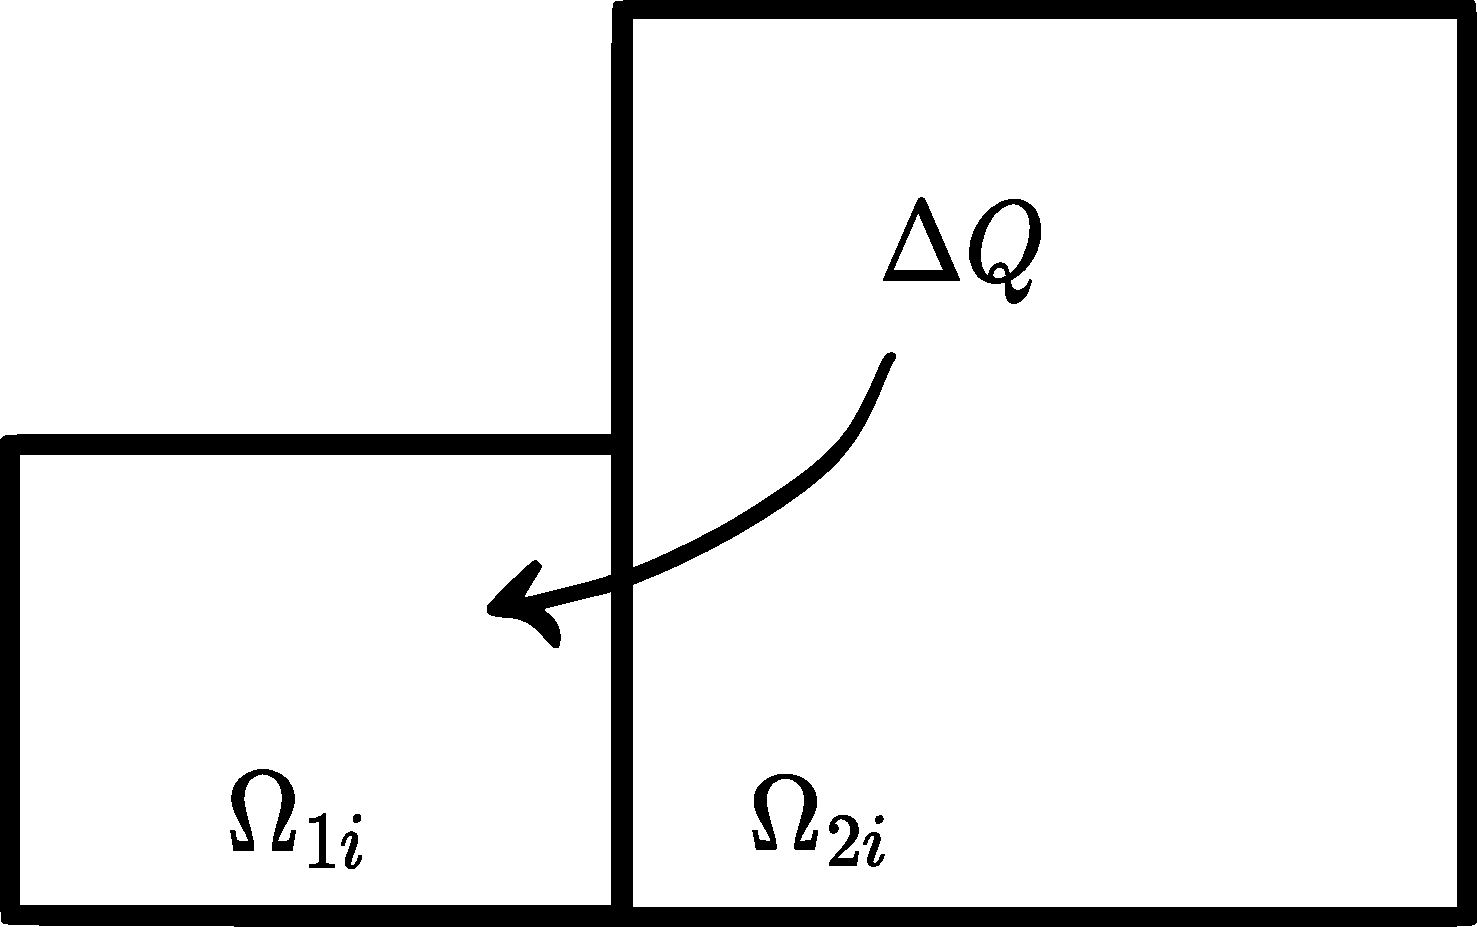
\includegraphics[scale=0.25]{fig/transf-calor.pdf}
\end{figure}

entonces hay $\Omega_{\text{tot},i}=\Omega_{1i}\cdot \Omega_{2i}$ estados accesibles al sistema combinado. Luego, la transferencia de calor ($\Delta Q$) hay $\Omega_{tot,f}=\Omega_{if}\cdot \Omega_{2f}$ estados accesibles al sistema combinado
\begin{equation}
  \Omega_{tot,f}>\Omega_{tot,i}
\end{equation}
En términos de la entropia:
\begin{equation}
  S_{1i}=k\log \Omega_{1i},\qquad  S_{2i}=k\log \Omega_{2i}
\end{equation}
Luego,
\begin{align}
  S_{tot,i}&=k\log \Omega_{tot,i}\\
  &=k\log (\Omega_{1i}\cdot \Omega_{2i})\\
  &=k\log (\Omega_{1i})+k\log (\Omega_{2i})
\end{align}
Así,
\begin{equation}
  S_{tot,i}=S_{1i}+S_{2i}
\end{equation}
Se concluye que la entropía es extensiva.

Notemos ademas que
\begin{equation}
  \Omega_{tot,f}>\Omega_{tot,i}\quad \Rightarrow \quad S_{tot,f}>S_{tot,i}
\end{equation}
es decir, la entropía aumenta en un proceso  de transferencia de calor.
\end{ej}

¿Cuál es la condición de equilibrio para que termine un proceso de transferencia de calor?

Cuando ambos sistemas quedan a la misma \textbf{temperatura}. Para definir temperatura, consideremos que en el nuevo equilibrio térmico:
\begin{equation}
  \left(\pdv{S_1}{U}\right)_{N,V}=-\left(\pdv{S_2}{U}\right)_{N,V}
\end{equation}
\begin{itemize}
	\item La energía interna $U$ cambia en ambos sistemas
	\item La ganancia $\Delta U_1$ en el sistema 1 es igual a la perdida $\Delta U_2$ en el sistema 2 (conservación de la energía).
	\begin{equation}
  \Delta U_1+\Delta U_2=0
\end{equation}
\item La entropía total aumenta, al cambiar $U$. Luego, $\Delta U$ deja de fluir cuando $S_{tot}$ deja de cambiar.
\item Se puede demostrar que el proceso continua hasta que (de lo anterior)
\begin{equation}
	\boxed{\left(\pdv{S_1}{U}\right)_{N,V}=-\left(\pdv{S_2}{U}\right)_{N,V}}
\end{equation}
\end{itemize}

Cuando
\begin{equation}
  \left(\pdv{S_1}{U}\right)_{N,V}=-\left(\pdv{S_2}{U}\right)_{N,V}
\end{equation}
entonces
\begin{equation}
  \left(\pdv{S_{tot}}{U}\right)_{N,V}=\left(\pdv{(S_1+S_2)}{U}\right)_{N,V}=\left(\pdv{S_1}{U}\right)_{N,V}+\left(\pdv{S_2}{U}\right)_{N,V}=0
\end{equation}
Luego,
\begin{equation}
\boxed{  \left(\pdv{S_{tot}}{U}\right)_{N,V}=0}
\end{equation}
y la entropía deja de aumentar con la transferencia de calor. Luego, el proceso se detiene. Así, conviene definir la temperatura $T$:
\begin{equation}
  \boxed{\frac{1}{T}=\left(\pdv{S}{U}\right)_{N,V}}\qquad \text{Al aumentar $T$ aumenta $U$.}
\end{equation}
Notamos que
\begin{equation}
  T_1=T_2\quad\Rightarrow\quad \frac{1}{T_1}=\frac{1}{T_2}\quad\Rightarrow \quad\left(\pdv{S_1}{U}\right)_{N,V}=\left(\pdv{S_2}{U}\right)_{N,V}
\end{equation}

\begin{cor}
	La transferencia de calor ocurre por gradiente de temperatura (el calor fluye desde e sistema de mayor temperatura hacia el de menor temperatura, asta que las temperaturas sean iguales).
\end{cor}

\subsection{Probabilidad de una configuración y factor de Boltzmann}
De la definición clásica de probabilidad, se tiene
\begin{equation}
  P=\frac{\# \text{casos favorables}}{\# \text{casos posibles}}
\end{equation}
El cuociente entre la probabilidad de dos estados macroscópicos es igual al cociente de sus \textit{degeneraciones.}

Considere un sistema \textit{pequeño} de 2 estados, $S_p$ y un sistema \textit{grande} o reservorio térmico $S_r$. Sea $U_0$ la energía del sistema combinado y $U_p$ la energía del sistema pequeño. Suponga que la energía del sistema $U_p$ puede ser $U_p=\epsilon$ y $U_p=0$.
\begin{itemize}
	\item Para $U_p=0$,\quad $U_r=U_0$\quad ($U_r$ energía del reservorio térmico)
	\item Para $U_p=\epsilon$,\quad $U_r=U_0-\epsilon$
\end{itemize}
El cociente entre las probabilidades esta dado por
\begin{equation}\label{1.1}
  \frac{P(\epsilon)}{P(0)}=\frac{\Omega(U_0-\epsilon)}{\Omega(U_0)}=\frac{e^{\frac{S}{k}(U_0-\epsilon)}}{e^{\frac{S}{k}(U_0)}}=\frac{\text{Prob. del $S_p$ con energía $\epsilon$}}{\text{Prob. del $S_p$ con energía $0$}}
\end{equation}
Luego, $\Omega(U)$ es la degeneración del reservorio térmico con energía $U$.

Expandiendo en serie de Taylor 
\begin{equation}
  S(U_0-\epsilon)\approx S(U_0)-\epsilon\left(\pdv{S}{U_0}\right)=S(U_0)-\frac{\epsilon}{T}
\end{equation}
Reemplazando en la exponencial de \eqref{1.1},
\begin{equation}
  \boxed{\frac{P(\epsilon)}{P(0)}\approx e^{-\frac{\epsilon}{kT}}}
\end{equation}
Conocido como el \textbf{factor de Boltzmann}.

La probabilidad relativa entre 2 estados escala como la exponencial de menos la diferencia de energía dividida por $kT$.

\begin{equation}
  	\textbf{Mientras más energético un estado, menos probable.}
\end{equation}

































\section{Clase 2}\label{clase:2}
\subsection{Entropía, ignorancia y teorema ergódico}
\begin{tcolorbox}
	\textbf{Principio de máxima entropía}: La configuración de un sistema desde el punto de vista macroscópico, es tal que maximiza la entropía, dada una serie de restricciones.
\end{tcolorbox}

Considere un número grande de sistemas idéntcos ($N_s\to \infty$), cada uno de los cuales puede estar en un estado específico.

Sea $n_i$ el número de sistemas que están en el estado $i$. Definimos la ignorancia $I$ (o la degeneración $\Omega$) como el número de formas de arreglar el sistema conjunto dado $\{n_i\}$ (factor multinomial)
\begin{equation}
  \boxed{I=\frac{N_s!}{n_0!n_1!\cdots},\qquad \sum_i n_i=N_s}
\end{equation}
\begin{ej}
	10 dados, cada uno puede estar en 6 estados. Luego, de tirarlos se obtiene que
	\begin{align}
  n_1&=4\\
  n_2&=3\\
  n_3&=0\\
  n_4&=0\\
  n_5&=0\\
  n_6&=3
\end{align}
entonces la configuración del sistema dada esta ignorancia es
\begin{equation}
  I=\frac{10!}{4!3!3!}
\end{equation}
\end{ej}
Esta ignorancia considera que sólo se conocen las poblaciones de los estados (cuantos sistemas hay en cada estado) y el número total de sistemas, pero que \textit{no es posible distinguir} entre sistemas que están en un mismo estado.

Buscamos una configuración (conjunto de poblaciones de estados) que maximice la ignorancia, sujeto a la restricción
\begin{equation}\label{2.1}
  \sum _i n_i=N_s
\end{equation}
Definimos\footnote{Cantidad extensiva. Maximizar $I$ implica maximizar $S$ (ya que el $\ln$ es monótono.) $\ln I \uparrow=S\uparrow$}
\begin{equation}
  \boxed{S=k\ln I}
\end{equation}
Entonces \begin{equation}\label{2.S}
  S=k\ln\left(\frac{N_s!}{n_0!n_i\cdots}\right)=k[\ln(Ns!)-\sum_i\ln(n_i!)]
\end{equation}
sujeto a \eqref{2.1}.

\textbf{Aproximación de Stirling:}
\begin{equation}\label{Stearling}
  \boxed{\ln(n!)\approx n\ln(n)-n}
\end{equation}

En efecto,
\begin{align}
  \ln(n!)=\ln(1\cdot 2\cdots n)&=\sum_i^n\ln(i)\approx\int_1^n\ln(x)\dd x\\
  &=\eval{x\ln x-x}_1^n\\
  &=(n\ln n-n)-(\cancelto{0}{\ln(1)}-1)\\
  &=n\ln n-n+1\\
  &=n\ln n-(n-1)\\
  &\approx n\ln n-n,\qquad \text{para $n\gg 1$}
\end{align}
Usando la aproximación de Sterling en \eqref{2.S}
\begin{align}
  S&\approx k\left[(N_s\ln(N_s)-\cancel{N_s})-\sum_i (n_i\ln(n_i)-\cancel{n_i})\right]\\
  &=k\left[N_s\ln(N_s)-\sum_in_i\ln(n_i)\right]
\end{align}
donde usamos que $N_s=\sum_i n_i$.

Dado $N_s$ fijo, buscamos $\{n_i\}$ que maximice $S$ sujeto a \eqref{2.1}. Como queremos maximizar utilizamos \textbf{multiplicadores de Lagrange}\footnote{Recordar que para una restricción holonómica $f(\{n_i\})=0$ se incluye $\lambda f$.}.
\begin{equation}
  S_{\{\sum_in_i=N\}}=k\left[N_s\ln(N_s)-\sum_in_i\ln(n_i)+\lambda \left(\sum_in_i-N_s\right)\right]
\end{equation}
Ahora
\begin{equation}
  L=\frac{S}{N_sk},\qquad \mu=\frac{\lambda}{k}
\end{equation}
Nos queda 
\begin{equation}
  L=\ln(N_s)-\sum_i\left(\frac{n_i}{N_s}\right)\ln(n_i)+\mu\left[\sum_i\left(\frac{n_i}{N_s}\right)-1\right]
\end{equation}
Definimos la probabilidad de que en la configuración total, un sistema cualquiera este en el estado $i$ como
\begin{equation}\label{sum Pi1}
  P_i=\frac{n_i}{N_s}
\end{equation}
Reescribimos
\begin{equation}
  \ln(n_i)=\ln\left(\frac{n_i}{N_s}N_s\right)=\ln(P_i)+\ln(N_s)
\end{equation}
Reemplazamos
\begin{align}
  L&=\ln(N_s)-\sum_i P_i\left(\ln(P_i)+\ln(N_s)\right)+\mu\left[\sum_i P_i-1\right]\\
  &=\ln(N_s)-\sum_iP_i\ln(P_i)-\sum_i P_i\ln(N_s)+\mu\left[\sum_i P_i-1\right],\qquad \sum_iP_i=1\\
  &=\cancel{\ln(N_s)}-\sum_iP_i\ln(P_i)-\cancel{\ln(N_s)}+\mu\left[\sum_iP_i-1\right]
\end{align}
Nos queda
\begin{equation}\label{2.2}
  L=-\sum_iP_i\ln(P_i)+\mu\left[\sum_i P_i-1\right]
\end{equation}
Las variables dinámicas son $\{P_i,\lambda\}$. Maximizando $L$
\begin{align}
  \pdv{L}{P_i}&=0\\
  \pdv{L}{\mu}&=0
\end{align}
Ahora, de \eqref{2.2},
\begin{align}
  \pdv{L}{P_i}&=-(\ln P_i+1)+\mu =0\label{2.3} \\
  \pdv{L}{\mu}&=\sum_i P_i=1
\end{align}
donde $\mu$ es constante. De \eqref{2.3},
\begin{equation}
  P_i=e^{\mu-1}=P,\qquad \sum_i P =1
\end{equation}
es decir, \corr{en la configuración que maximiza la entropía, cada estado es igualmente probable} (la probabilidad es igual a una constante que no depende de $i$).

Hay $s$ estados posibles, luego
\begin{equation}
  sP=1\quad \Rightarrow \qquad P=\frac{1}{s}
\end{equation}

Esto implica que la probabilidad de cada estado en la configuración de máxima entropía es
\begin{equation}
  \frac{1}{\# \text{ estados posibles}}
\end{equation}
luego,
\begin{equation}
  \boxed{n_i=N_sP=\frac{N_s}{s}},\qquad \Rightarrow \qquad \sum_{i=1}^sn_i=N_s
\end{equation}
La ocupación de cada estado, en la configuración que maximiza la entropía (y que maximiza la ignorancia o degeneración) es igual al número de sistemas presentes dividido en el número de estados posibles. 













































\section{Clase 3}\label{clase:3}
\subsection{Principio fundamental de la termodinámica}
\begin{tcolorbox}
La configuración total \textbf{maximiza la entropía}, sujeta a restricciones macroscópicas que dependen de las cantidades fluctuantes conservadas.
\end{tcolorbox}

En la Clase \ref{clase:2} vimos que si suponemos una configuración $N_s$ sistemas los que pueden existir en $m$ estados diferentes, siendo sus ocupaciones el conjunto:
\begin{equation}
  \{n_i\}_{i=1}^m
\end{equation}
la ignorancia $I$, o degenerancia $\Omega$ esta dada por
\begin{equation}
  \boxed{I=\frac{N_s!}{\Pi_{i=1}^mn_i}}
\end{equation}
Se define la entropía $S$ como
\begin{equation}
  \boxed{S=\kappa \ln I}
\end{equation}
Usando Stearling, se tiene
\begin{align}
  \frac{S}{\kappa}=N_s\ln (Ns)-Ns-\left[\sum_{i=1}^m\left(n_i\ln (n_i)-n_i\right)\right]
\end{align}
Usando que $\sum_{i=1}^m=N_s$,
\begin{align}
  \frac{S}{\kappa}&=N_s\ln (Ns)-\summ n_i\ln(n_i)\quad /\frac{1}{N_s}\\
  \frac{S}{\kappa N_s}&=\ln(N_s)-\summ\left(\frac{n_i}{N_s}\right)\ln (n_i)\label{3.1si}
\end{align}
Usando que
\begin{equation}
  \ln(n_i)=\ln\left(\frac{n_i}{N_s}N_s\right)=\ln\left(\frac{n_i}{N_s}\right)+\ln(N_s)
\end{equation}
reemplazando en \eqref{3.1si},
\begin{align}
  \frac{S}{\kappa N_s}&=\ln (N_s)-\summ\left(\frac{n_i}{N_s}\right)\left[\ln(\frac{n_i}{N_s})+\ln (N_s)\right]\\
  &=\ln(N_s)-\summ \left(\frac{n_i}{N_s}\right)\ln(\frac{n_i}{N_s})-\summ \left(\frac{n_i}{N_s}\right)\ln(N_s)
\end{align}
pero usando \eqref{sum Pi1}
\begin{equation}
  \summ \left(\frac{n_i}{N_s}\right)=\summ P_i=1
\end{equation}
así,
\begin{align}
  \frac{S}{\kappa N_s}&=\ln(N_s)-\summ \left(\frac{n_i}{N_s}\right)\ln(\frac{n_i}{N_s})-\ln(N_s)\\
  &=-\summ\left(\frac{n_i}{N_s}\right)\ln(\frac{n_i}{N_s})
\end{align}
\begin{equation}
  \Rightarrow \boxed{\frac{S}{\kappa N_s}=-\summ\left(\frac{n_i}{N_s}\right)\ln(\frac{n_i}{N_s})}
\end{equation}
Definimos la probabilidad de que un sistema esté en el estado $i$ como \eqref{sum Pi1}
\begin{equation}
\boxed{P_i=\frac{n_i}{N_s}}
\end{equation}
y la entropia de Shannon como
\begin{equation}
  \boxed{\frac{S}{\kappa N_s}=-\summ P_i\ln (P_i)}
\end{equation}
Por el principio fundamental del termodinámica, sin imponer conservación de las cantidades conservadas. Pero considerando
\begin{equation}
  \summ P_i=1
\end{equation}
maximizamos la entropía
\begin{align}
  L&=-\summ P_i\ln(P_i)+\lambda\left(\summ P_i-1\right)
\end{align}
donde $\lambda$ son los multiplicadores de Lagrange y $\summ P_i-1$ es una restricción holonómica.
\begin{align}
  \left(\pdv{L}{P_i}\right)_{P_i,\lambda}&=0,\qquad \forall i\neq j\label{3.1}\\
  \left(\pdv{L}{\lambda}\right)_{P_i}&=0\label{3.2}
\end{align}
De \eqref{3.1}
\begin{align}
  -\ln(P_i)-P_i\frac{1}{P_i}+\lambda&=0\\
  \Rightarrow \ln(P_i)&=\lambda-1
\end{align}
obtenemos
\begin{equation}
  P_i=e^{\lambda-1}
\end{equation}
notemos que esta expresión es independiente de $i$.
De \eqref{3.2},
\begin{align}
  \summ P_i-1&=0\\
 \Rightarrow \summ P_i&=1\\
 \Rightarrow \summ P_i&=mP=me^{\lambda-1}=1
\end{align}
luego
\begin{equation}
  P_i=\frac{1}{m}\quad \Rightarrow\quad n_i=\frac{N_s}{m}\quad\Rightarrow\quad \lambda=-\ln(n)+1
\end{equation}
\corr{Sin imponer restricciones de conservación, excepto que la suma de las probabilidades de los estados es igual a $1$, obtenemos que la configuración que maximiza la entropía es la distribución uniforme de estados equiprobables}. La ocupación de cada uno de los $m$ estados es:
\begin{equation}
  \boxed{n_i=\frac{N_s}{m}}
\end{equation}

\bako{Si imponemos conservación de la energía},
\begin{itemize}
	\item Cada estado $i$ tiene energía $E_i$
	\item Si las ocupaciones de dichos estados son $n_i$, la energía total de la configuración es
	\begin{equation}
  E=\summ E_in_i
\end{equation}
\item Agregamos la conservación de $E$ como una restricción al funcional de entropía.
\end{itemize}

Sea $S_E$ la restricción
\begin{equation}
  S_E=\b \k \left(E-\summ E_in_i\right)
\end{equation}
con $\b$ un multiplicador de Lagrange. Consideremos
\begin{equation}
  L_E=\frac{S_E}{\k N_s}=\b \left(\bar{E}-\summ E_iP_i\right)
\end{equation}
donde 
\begin{equation}
  \bar{E}=\frac{E}{N_s}
\end{equation}
es la energía promedio del sistema.

Luego, nuestro Lagrangeano queda
\begin{equation}
  L=-\summ P_i\ln(P_i)-\lambda \left(\summ P_i-1\right)-\b \left(\summ E_iP_i-\bar{E}\right)
\end{equation}
Ahora,
\begin{align}
  \left(\pdv{L}{P_i}\right)_{P_i,\lambda}&=\ln(P_i)-1-\lambda-\b E_i\\
  \left(\pdv{L}{\b}\right)_{P_i,\lambda}&=\summ E_iP_i=\bar{E}\\
  \left(\pdv{L}{\lambda}\right)_{P_i,\b}&=\summ P_i=1
\end{align}
\begin{equation}
  \ln(P_i)=-\lambda-\b E_i-1
\end{equation}
entonces
\begin{equation}
\boxed{  P_i=e^{-\lambda-\b E_i-1}}
\end{equation}
\begin{align}
  P_i&=e^{-\lambda-1}e^{\b E_i}\\
  \summ P_i&=1\Rightarrow \summ e^{-\lambda-1}e^{-\b E_i}=1\\
  \Rightarrow (e^{-\lambda-1})\summ e^{\b E_i}=1\\
  \Rightarrow e^{-\lambda-1}&=\frac{1}{\summ e^{-\b E_i}}
\end{align}
tenemos
\begin{equation}
  \boxed{P_i=\frac{e^{-\b E_i}}{\summ e^{-\b E_i}}}\quad \Rightarrow\quad \boxed{z=\summ e^{-\b E_i}}\quad \Rightarrow\quad \boxed{P_i=\frac{e^{-\b E_i}}{z}}
\end{equation}
En el caso de imponer conservación de la energía, la configuración solo puede explorar conjuntos de ocupaciones $\{n_i\}_{i=1}^n$ que tengan la misma energía total.

En general, la configuración equiporbable no es alcanzable necesariamente, ya que tiene una energá total particular, que puede ser diferente a la energía inicial dada.

En particular, la energía de la configuración equiprobable es
\begin{align}
  E_{\rm equi}&=\summ E_in_i\\
  &=\summ E_i\frac{N_s}{n}
\end{align}
esto implica
\begin{equation}
  \boxed{E_{\rm equi}=\frac{N_s}{n}\summ E_i}
\end{equation}
Si $E\neq E_{\rm equi}$, la configuración equiprobable es inalcanzable. Para $E$ consevado, la probabilidad de que un sistema esté en el estado $i$ es
\begin{equation}
 \boxed{P_i=\frac{e^{-\b E_i}}{z}}
\end{equation}
donde
\begin{equation}
\boxed{  z=\summ e^{-\b E_i}}
\end{equation}
se conoce como la \textbf{función de partición} y $e^{-\b E_i}$ se llama \textbf{factor de Boltzmann} y tiene la interpretación de un peso estadistico.
\begin{itemize}
	\item $z$ es la suma de todos los pesos
	\item La ocupación del estado $i$ es
	\begin{equation}
\boxed{  n_i=N_sP_i=N_s\frac{e^{-\b E_i}}{z}}
\end{equation}
\end{itemize}

\subsection{Conservación de energía y carga $Q$}
$Q$ puede ser número de partículas, carga eléctrica, momento angular, magnetización, etc...

$Q$ es una cantidad macroscópica, extensiva, diferente de $(E,V,S)$ que caracteriza la configuración macroscópica y que se conserva entre las distintas configuraciones.

El Lagrangeano se verá
\begin{equation}
  L=-\summ P_i\ln(P_i)-\underbrace{\lambda \left(\summ P_i-1\right)}_{\summ P_i=1}-\underbrace{\b\left(\summ E_iP_i-\bar{E}\right)}_{\text{Conservación de la energía}}-\underbrace{\b \m\left(\summ Q_iP_i-\bar{Q}\right)}_{\text{Conservación de la carga}}
\end{equation}
con $\bar{Q}$ la carga promedio del sistema.

Ahora
\begin{align}
  -\ln(P_i)-1-\lambda-\b E_i-\b\m Q_i&=0\\
  P_i=e^{\lambda-1-\b E_i-\b\m Q_i}&=0\\
  P_i&=e^{-\lambda-1}e^{-\b(E_i+\m Q_i)}
\end{align}
usando $\summ P_i=1$,
\begin{align}
  \summ e^{-\b (E_i+\m Q_i)}=\frac{1}{e^{-\lambda-1}}
\end{align}
Definimos
\begin{equation}
\boxed{  Z_{\rm GC}=\summ e^{-\b (E_i+\m Q_i)}}
\end{equation}
entonces
\begin{equation}
 \boxed{ P_i=\frac{e^{-\b (E_i+\m Q_i)}}{Z_{\rm GC}}}
\end{equation}
donde $Z_{\rm GC}$ es la \textbf{función partición Gran Canónica} y corresponde a la suma de los pesos estadisticos $e^{-\b (E_i+\m Q_i)}$. $n_i=N_sP_i$ es la ocupación de los estados.

\subsection{Ensambles, funciones de partición y potenciales termodinámicos}
\begin{itemize}
	\item Maximizando la entropía, sujeto a diferentes restricciones, hemos encontrado la probabilidad de ocupación de los estados posibles de los sistemas.
	\item Dichas probabilidades pueden interprearse como pesos estadisticos para cada estado, normalizados por una función partición.
	\item Dependiendo de las cantidades conservadas las funciones partición son ditintas.
	\item El conjunto de configuraciones posibles dadas las restricciones, definen la noción de ensamble.
	\item A cada tipo de ensamble, especificado por ciertas cantidades conservadas, le corresponde una función partición.
\end{itemize}


\begin{center}
\begin{tabular}{|c|c|c|c|c|}
\hline
  Ensamble & Can. fluctuantes conservadas & Can. fijas & Función partición & Pot. termodinámico  \\
  \hline\hline
  Microcanónico & ----- & $E,V,Q$& $I$& $S$ \\\hline
  Canónico&$E$ &$T,V,Q$&$z=\summ e^{-\b E_i}$&$F$\\\hline
  Gran Canónico&$E,Q$&$T,V,\m$&$z=\summ e^{-\b(E_i+\m Q_i)}$&$\Omega_{\rm GC}$\\\hline
  Isobárico&$E,V$&$T,P,Q$&&\\\hline
\end{tabular}
\end{center}
donde
\begin{equation}
  \b=\frac{1}{T}
\end{equation}

Notas que $\b,\m$ y $P$ son intensivas.

$T=\frac{1}{\b}$ viene dado por el multiplicador de Lagrange asociado a la conservación de energía.






































\section{Clase 4}
\subsection{Ensamble micro-canónico}
De la Clase \ref{clase:3} vimos que en el ensamble micro-canónico
\begin{equation}
  P_i=\frac{n}{N_s}
\end{equation}
cada estado equiprobable. $(E,V,Q)$ están fijos.

\subsection{Ensamble canónico}
%En el \textbf{ensamble canónico},
\begin{align}
  P_i&=\frac{1}{Z_{\rm C}}e^{-\b E_i}\\ Z_{\rm C}&=\summ e^{-\b E_i}\\ \bar{E}&=\summ P_iE_i \quad \text{(restricción)}\\
  \b&=\frac{1}{T}
\end{align}
$(T,V,Q)$ están fijos. $\bar{E}$ es fluctuante.

\subsection{Ensamble Gran Canónico}
%En el \textbf{ensamble Gran Canónico},
\begin{align}
  P_i&=\frac{1}{Z_{\rm GC}}e^{-\b E_i-\a Q_i}\\
  Z_{\rm GC}&=\summ e^{-\b E_i-\a Q_i}\\
  \bar{E}&=\summ P_iE_i\label{4.1}\\
  \bar{Q}&=\summ P_iQ_i\label{4.2}\\
  \b&=\frac{1}{\k T}\\
  \a&=-\frac{\m}{\k T}
\end{align}
Aquí \eqref{4.1} y \eqref{4.2} son restricciones. $(T,V,\m)$ están fijos. $\bar{E}$ y $\bar{Q}$ son fluctuantes.

La configuración de cada ensamble \textbf{maximiza la entropía} sujeta a las restricciones correspondientes, implementadas mediante multiplicadores de Lagrange.

\begin{tcolorbox}
	A partir de ahora introduciremos la siguiente \textbf{notación}, 
	\begin{itemize}
		\item $T$: temperatura
		\item $\m$: potencial químico
		\item $z$: función partición
		\item $\k$: Constante de Boltzmann
	\end{itemize}	
\end{tcolorbox}

Partiendo de la función partición (considerando el ensamble Gran Canónico por generalidad), se tiene
\begin{align}
  \bar{E}&=\summ P_iE_i=\frac{\summ E_ie^{-\b E_i-\a Q_i}}{Z}\\
  &=-\left(\pdv{\b}\ln(Z)\right)_\a\label{E=partial-beta}
\end{align}
\begin{equation}
\boxed{  \bar{E}=\k T^2\left(\pdv{T}\ln(Z)\right)_{\m/T}}
\end{equation}
con \begin{equation}
  \b =\frac{1}{\k T}\quad \Rightarrow\quad \pdv{\b }=-T^2\kappa\pdv{T}
\end{equation}
también tenemos
\begin{align}
  \bar{Q}&=\frac{\summ Q_ie^{-\b E_i-\a Q_i}}{Z}\\
  &=-\left(\pdv{\a }\ln(Z)\right)_\b 
\end{align}
\begin{equation}
 \boxed{ \bar{Q}=\k T\left(\pdv{\m }\ln(Z)\right)_T}
\end{equation}
con
\begin{equation}
  \a =\frac{\m }{\k T}\quad \Rightarrow\quad \pdv{\a }=\k T\pdv{\m }
\end{equation}
También es posible relacionar la función partición con la entropía
\begin{align}
  S&=-\k \summ P_i\ln(P_i)\\
  &=\k\summ P_i(\ln(Z)+\b E_i+\a Q_i)\\
  &=\k \left(\ln(Z)+\b \bar{E}+\a \bar{Q}\right)
\end{align}
luego
\begin{equation}
\boxed{  S=\k \ln(z)+\frac{\bar{E}}{T}-\frac{\m \bar{Q}}{T}}\quad \Rightarrow\quad \boxed{-\k T\ln(z)=\bar{E}-TS-\m Q}
\end{equation}

Para los diferentes ensambles, existen potenciales termodinámicos definidos en términos de $\ln(Z)$. \footnote{Los signos y los factores delante son por razones históricas, desafortunadamente. :(}

\textbf{Potencial Gran Canónico}
\begin{equation}
  \Omega_{\rm GC}=-\k T\ln(Z_{\rm GC})=\bar{E}-TS-\m\bar{Q}
\end{equation}

\textbf{Energía libre de Hemholtz}
\begin{equation}
  F=-\k T\ln(Z_{\rm C})=\bar{E}-TS\quad (Q_i=0)
\end{equation}

Existen relaciones entre los potenciales termodinámicos de los diferentes ensambles. Por ejemplo, definiendo la \textbf{densidad de estados}
\begin{equation}
  \r(Q,E)=\frac{e^{S(Q,E)/\kappa}}{\delta E}	
\end{equation}
$\r(Q,E)$ cuenta el número de estados con carga $Q$ y energía entre $E$ y $E+\delta E$. De aquí podemos obtener la energía libre de Hemholtz como
\begin{equation}
  F(Q,T)=-\k T\ln(Z_{\rm C})=-\k T\ln\int\dd E\r(Q,E)e^{-E/\k T}
\end{equation}
Finalmente el potencial Gran Canónico, puede calcularse como
\begin{equation}
  \Omega_{\rm GC}(\m,T)=\k T\ln(\zgc)=-T\ln\left(\sum_Qe^{-F(Q,T)/\k T}e^{\m Q/\k T}\right)
\end{equation}

\subsection{Ensamble isobárico-isotérmico}
En el ensamble isobárico-isotérmico $(T,P,Q)$ son constantes y $(\bar{E},\bar{V})$ son fluctuantes.

Notemos que $V$ es una cantidad extensiva (proporcional al número total de sistemas $N_s$). Si no hay restricciones entre sistemas, el potencial Gran Canónico por unidad de volumen es independiente del volumen (cada región es igual a cualquier otra).

Por último, la presión se define como menos la derivada del potencial termodinámico (Gran Canónico) con respecto al volumen. Luego,
\begin{equation}
  \Omega_{\rm GC}=\o_{\rm GC}V
\end{equation}
donde $\o_{\rm GC}$ es el potencial Gran Canónico por unidad de volumen. Se sigue que
\begin{equation}
  \pdv{\ogc}{V}=0
\end{equation}
así,
\begin{equation}
  P=\pdv{V}\Ogc=-\ogc=-\frac{\Ogc}{V}
\end{equation}
Entonces
\begin{equation}
\boxed{  \Ogc=-PV=-\k T\ln(\zgc)=E-TS-\m Q}
\end{equation}
\begin{equation}\label{4.3}
\boxed{  PV=TS-E+\m Q}
\end{equation}
Se define $G$, la \textbf{enegía libre de Gibbs}, como\footnote{se deriva de \eqref{4.3}}
\begin{equation}
\boxed{  G=\m Q=E-TS+PV}
\end{equation}

$G$ es el potencial termodinámico del ensamble isobárico-isotérmico.

Además, podemos obtener la siguiente relación
\begin{equation}
\boxed{  E=TS-PV+\m Q}
\end{equation}
conocida como la \textbf{relación de Euler}.






























% Bibliography

%% [A] Recommended: using JHEP.bst file
%% \bibliographystyle{JHEP}
%% \bibliography{biblio.bib}

%% or
%% [B] Manual formatting (see below)
%% (i) We suggest to always provide author, title and journal data or doi:
%% in short all the informations that clearly identify a document.
%% (ii) please avoid comments such as "For a review'', "For some examples",
%% "and references therein" or move them in the text. In general, please leave only references in the bibliography and move all
%% accessory text in footnotes.
%% (iii) Also, please have only one work for each \bibitem.


\newpage
\bibliographystyle{JHEP}
\bibliography{biblio.bib}
\end{document}
